\documentclass[a4paper,12pt,notitlepage]{article}	% oneside : pour ne pas avoir de sauts de page

% Le fichier de preambule est comment aux fascicules de TP et de TD
\usepackage{helvet}
\renewcommand{\familydefault}{\sfdefault}

\usepackage{tocloft}
\usepackage{caption}
\usepackage{alltt}
\usepackage[dvipsnames,table]{xcolor}
\usepackage[french]{babel}
\usepackage[latin1]{inputenc}
\usepackage{amsmath,amsbsy,amssymb,empheq}
% \newtheorem{theo}{Th�or�me}   % Environnement theoreme
% \usepackage{amsfonts}
\usepackage{graphicx}
\usepackage{listings,comment}
\usepackage{tabularx} % Pour avoir des tableaux d'une largeur bien d�finie
\usepackage{multirow} % pour faire fusionner des lignes dans des tableaux
\usepackage[babel=true]{csquotes} % csquotes va utiliser la langue d�finie dans babel
\usepackage[rightcaption]{sidecap}% Pour utiliser SCfigure (figure encadree)
\usepackage[squaren,Gray]{SIunits} % pour avoir de jolies unit�s
\usepackage{enumitem}
\usepackage{hyperref}
\usepackage{color}
\usepackage{xifthen}
\usepackage[makeroom]{cancel}
\usepackage{csquotes}
\usepackage{subfig} % Pour avoir des sous-figures
\usepackage{bigints}
\usepackage{float}
\usepackage{icomma} 
\usepackage{textcomp} 

\usepackage{sectsty}
%\allsectionsfont{\color{blue}\itshape\underline}
% \sectionfont{\color{red}\itshape\selectfont}
\sectionfont{\color{red}}
\subsectionfont{\color{blue}}


\everymath{\displaystyle}



% Format des pages
%\pagestyle{headings}  
\oddsidemargin  -1cm
\evensidemargin -1cm
\textwidth 17cm % A ajuster pour les commentaires dans la marge
% \textwidth 18cm
\topmargin -2cm
\textheight 26cm
\makeatletter
\@addtoreset{chapter}{part}
\makeatother

\makeatletter
\newcommand*{\toccontents}{\@starttoc{toc}}
\makeatother


% -------------------------------------------------------------------------------

\newenvironment{etapes}{%
  \begin{itemize}
  \def\etape{\item[\textbullet] }
}{
  \end{itemize}
}

% fonction rectangle
\newcommand{\sinc}[0]{\mathrm{sinc}}

% quotation marks
\newcommand{\g}[1]{\og#1\fg}

% Rightarrow
\newcommand{\Ra}[0]{\Rightarrow}

\newcommand{\ora}[1]{\overrightarrow{#1}} 

\newcommand{\er}{\ensuremath{\va*{e}_{r}}}
\newcommand{\etheta}{\ensuremath{\va*{e}_{\theta}}}
\newcommand{\ephi}{\ensuremath{\va*{e}_{\varphi}}}
\newcommand{\vr}{\ensuremath{\va{r}}}

\newcommand{\ex}{\ensuremath{\va*{e}_{x}}}
\newcommand{\ey}{\ensuremath{\va*{e}_{y}}}
\newcommand{\ez}{\ensuremath{\va*{e}_{z}}}


% \noyau{C}{12}{6} pour le carbone
\newcommand{\noyau}[3]{\prescript{#2}{#3}{\mathrm{#1}}} 

\newcommand{\id}[1]{\mathrm{#1}}  

\newcommand{\mr}[2]{\multirow{#1}{*}{#2}}  
\newcommand{\mc}[3]{\multicolumn{#1}{#2}{#3}}  

% texte en couleur
\newcommand{\tc}[2]{\textcolor{#1}{#2}}
\newcommand{\tcb}[1]{\textcolor{blue}{#1}}
\newcommand{\tcr}[1]{\textcolor{red}{#1}}

\newcommand{\al}[0]{
\setlength{\abovedisplayskip}{0pt}
\setlength{\belowdisplayskip}{0pt}    
}

\newcounter{otheryear}
\setcounter{otheryear}{\the\year}
\ifthenelse{\cnttest{\month}{>}{6}}{\addtocounter{otheryear}{1}}{\addtocounter{otheryear}{-1}}
\def\semestre{\ifthenelse{\cnttest{\month}{>}{6}}{\the\year -\theotheryear}{\theotheryear -\the\year}}
\graphicspath{{Figures/}}

\usepackage{fancyhdr}
\fancypagestyle{thetitlepage}{
\fancyhead{} % clear all header fields
\fancyfoot{} % clear all footer fields
\renewcommand{\headrulewidth}{0pt}
\renewcommand{\footrulewidth}{0pt}
}



% Environnement ``reponse'' et questions
\usepackage{framed} % Pour encadrer du texte
\setlength{\FrameRule}{\fboxrule}
\setlength{\FrameSep}{3\fboxsep}

%\patchcmd\chapter{\null\vfil}{}{}{}
% Environnement ``question'' recupere du package ``exam.sty''
% compteur pour num�roter les questions � la suite dans un m�me TP.
\newcounter{numQuestion}
\newcommand{\resetQuestions}{\setcounter{numQuestion}{1}}
\resetQuestions 

\newenvironment{questions}[1][start=\thenumQuestion]%
{%
  \setlength{\leftmargini}{6pt}
  \setlength{\leftmarginii}{8mm}
  \setlength{\leftmarginiii}{10mm}
  \renewcommand{\labelenumi}{{\bf \theenumi.}}
  \renewcommand{\labelenumiii}{(\theenumiii)}

  % Cadre autour de l'environnement ``questions''
  % \begin{framed}\begin{enumerate}[#1]\addtolength{\itemsep}{2mm}
  % \def\question{\item}\let\ques\question}
  % {\end{enumerate}\end{framed}}
  % Pas de cadre autour de l'environnement ``questions''
  \begin{enumerate}[#1]\addtolength{\itemsep}{2mm}
  \def\question{\item}\let\ques\question
}%
{%
  \setcounter{numQuestion}{\theenumi}
  \addtocounter{numQuestion}{1}
  \end{enumerate}
}

\newenvironment{reponse}
{ %\leftskip1.5em
  \begin{framed}\color{blue}%
  }{%
%  \vspace{-2pt}% ajustement d'espacement en bas  
  \color{black}\end{framed}%
}

\newenvironment{reponsefigure} 
{ %\leftskip1.5em   
  \begin{figure}%
  }{% %  \vspace{-2pt}
  % ajustement d'espacement en bas    
  \end{figure}% 
}

\newenvironment{reponseSCfigure} 
{ %\leftskip1.5em
  \begin{SCfigure}%
  }{%
%  \vspace{-2pt}% ajustement d'espacement en bas  
  \end{SCfigure}%
}


% Commenter les lignes suivantes pour faire apparaitre les reponses
% \usepackage{versions}
% \excludeversion{reponse}

% \title{TP Geant4}
% \author{Calculatrice et documents non autorisés (sauf le document de la CRIIRAD) ; \\le barème est donné à titre indicatif.}
\date{}

%\citeindextrue

\usepackage{fancyhdr}

\renewcommand{\thispagestyle}[1]{} % do nothing

\begin{document}

% \pagestyle{fancy} 
% \lhead{Université Lyon 1 \\ M1 Physique \\UE \g{Interactions Rayonnements-Matière}} 
% \rhead{Année 2022-2023\\PHY1242M } %empty 
\title{TP Masterclass \g{Particle Therapy} \\ \small Planification de traitement avec matRad }
% \author{E. Testa}
\date{}

\maketitle

Ce TP a pour but de vous faire découvrir la planification de traitement de tumeurs cancéreuses par radiothérapie et de mettre en évidence les principaux avantages des irradiations par faisceaux de photons de protons et d'ions carbone.

\section{Préambule}

\paragraph{Lancement des logiciels X2Go et matRad}

Pour ce TP, nous allons utiliser un serveur de calcul sur lequel est installé le logiciel matRad. L'accès à ce serveur de calcul (sous Linux) s'effectue via le logiciel \g{X2Go}. 

\begin{itemize}
	\item Démarrer le logiciel X2go et créer un nouvelle session avec les informations (login/mdp) que l'on vous a envoyées. L'adresse IP du serveur est : 193.54.49.211 (cf. Figure~\ref{ConfigX2Go}).	Penser à définir le \textbf{type de session comme \g{XFCE}} (dernier menu en bas de la fenêtre de configuration).\footnote{Si une alerte de pare-feu apparaît, cliquer sur Annuler. Si un message d'alerte apparaît à propos d'une connexion à un nouveau serveur, cliquer sur Accepter.} Une fois la session définie, double-cliquer dessus pour obtenir la fenêtre de connexion avec login et mot de passe.
	\item Entrer ensuite votre login/mdp dans le menu d'ouverture de session
\end{itemize}

\begin{figure}[!htp]
  \centering
  \subfloat[Configuration de X2Go.]
  {\label{ConfigX2Go}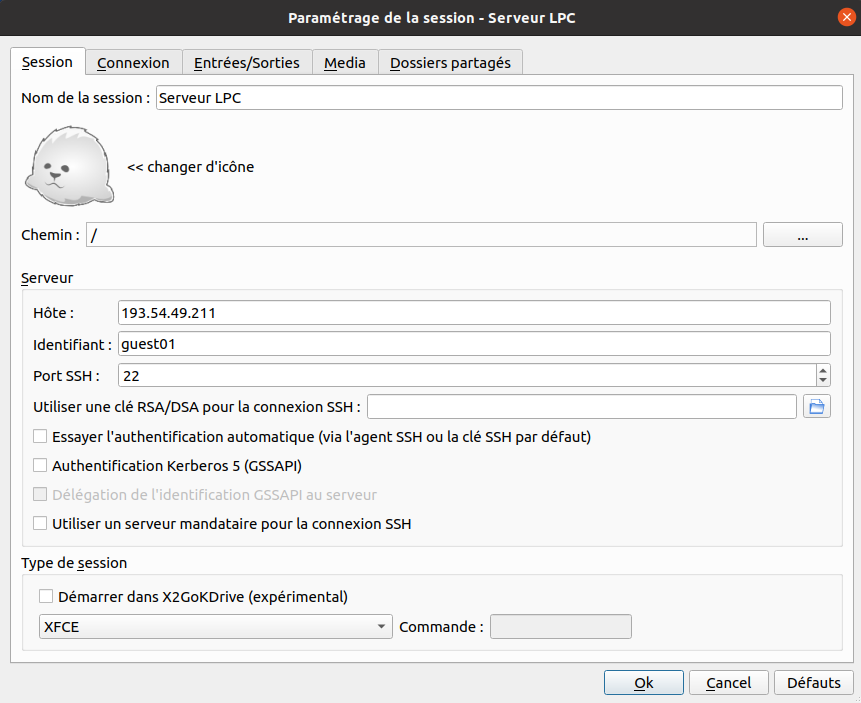
\includegraphics[height=.22\textheight]{./Figures/ConfigX2Go} }    
  \subfloat[Environnement de travail]{\label{Bureau}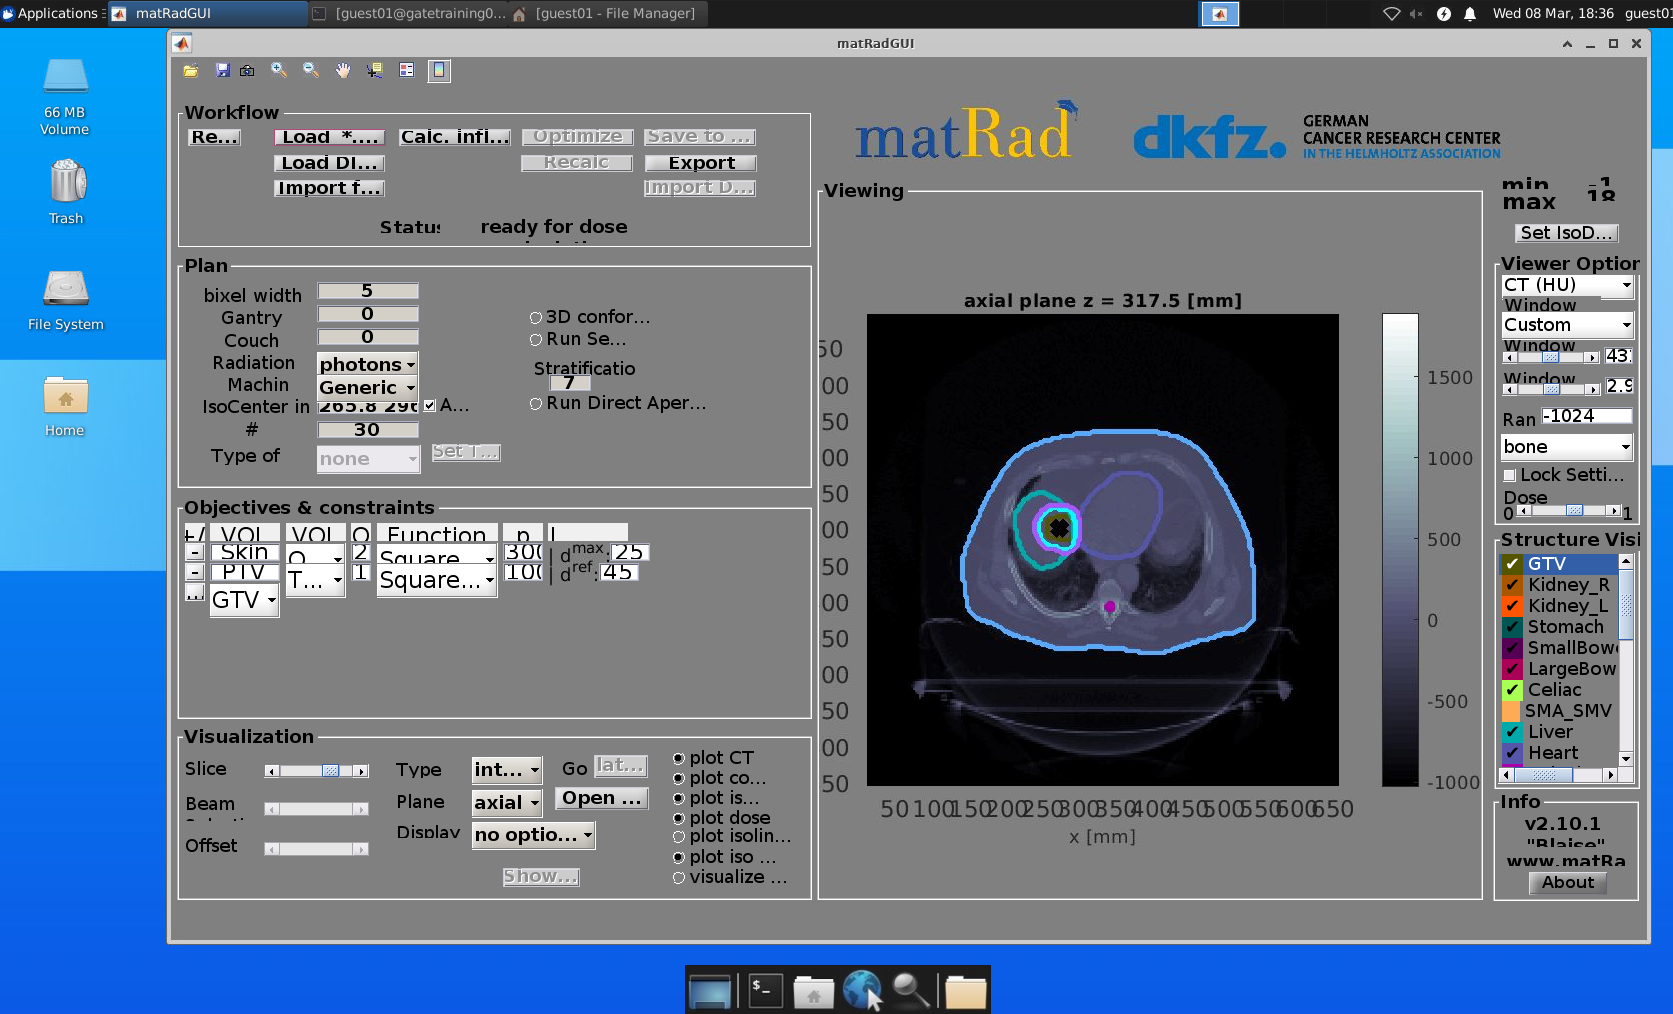
\includegraphics[height=.22\textheight]{./Figures/Bureau}}  
  \caption{Configuration de X2Go et environnement de travail.}
\end{figure} 	

Une fois dans l'environnement de travail (Figure~\ref{Bureau}) :
\begin{itemize}
	\item ouvrir un terminal (cliquer sur le deuxième icône à partir de la gauche, tout en bas du bureau)
	\item se placer dans le dossier \g{masterclass} en tapant : \texttt{cd masterclass}
	\item récupérer le programme d'analyse des données de sortie de matRad en tapant: \\ \texttt{git clone https://github.com/etesta/MasterclassPT\_Notebook}
	\item lancer le logiciel matRad en tapant : \texttt{matrad}
	\item \tcr{Bien penser à la fin du TP à se déconnecter proprement de X2Go : pour cela, sortir de la session (\g{Log out}) puis fermer X2Go.}
\end{itemize}


\section{Comparaison des traitements par faisceaux de photons, protons et ions carbone (tumeur du foie)}

Les objectifs de cet exercice sont les suivants :
\begin{itemize}
  \item  découvrir le logiciel,
  \item comparer les dépôts de dose des photons, des protons et des ions carbone avec un seul champ d'irradiation,
	\item tendre vers une planification de traitement photon réaliste avec plusieurs champs d'irradiation.
\end{itemize}




\begin{questions}
  
\question Charger le cas du patient atteint du foie via le bouton \textbf{Load *.mat (LIVER.mat)} (dossier \g{masterclass/patients}). Identifier les différents organes du patient en particulier le foie, le volume cible et les organes à risque en utilisant les différentes vues du patient (\g{axial, sagittal, coronal} dans le menu \textbf{\g{visualization}}). Sélectionner les volumes suivants dans la liste des \g{structures} :  c\oe ur (heart), estomac (stomach), foie (liver), peau (skin) et le volume cible planifié (PTV).

\begin{reponse}
	Les vues axiale, coronale et sagitale :
	
  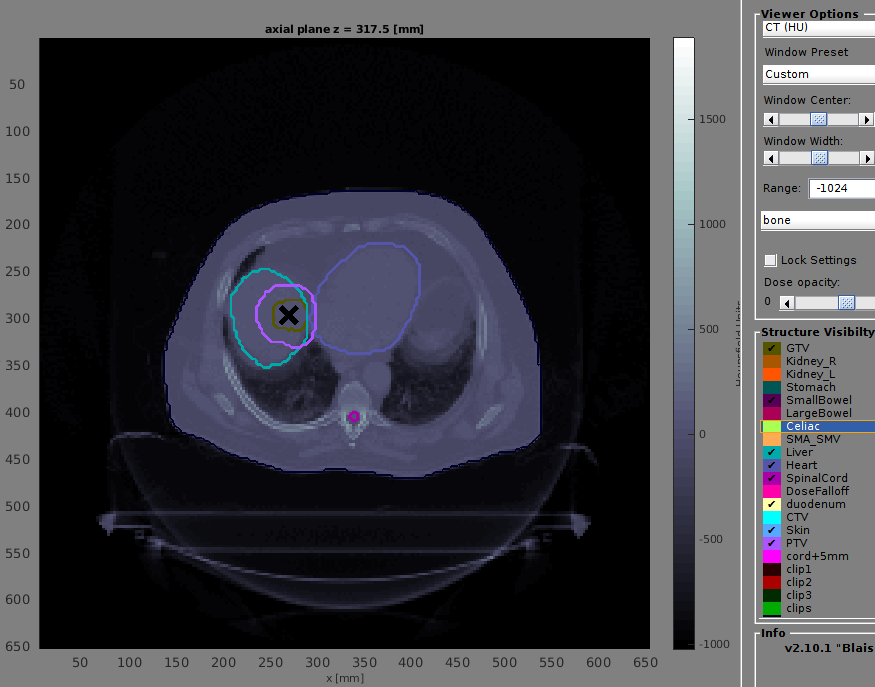
\includegraphics[height=.2\textheight]{./Figures/LiverAxial} \quad 
	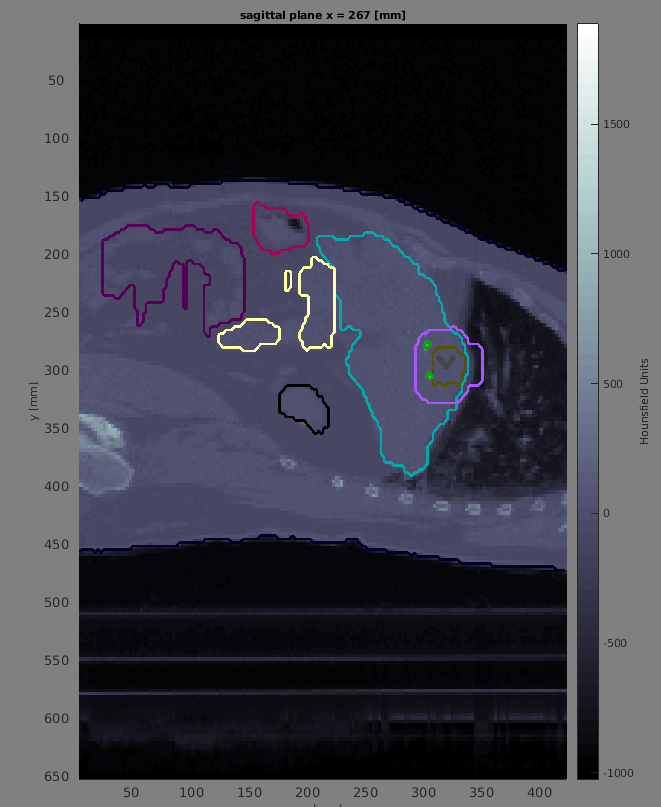
\includegraphics[height=.2\textheight]{./Figures/LiverSagittal} \quad
	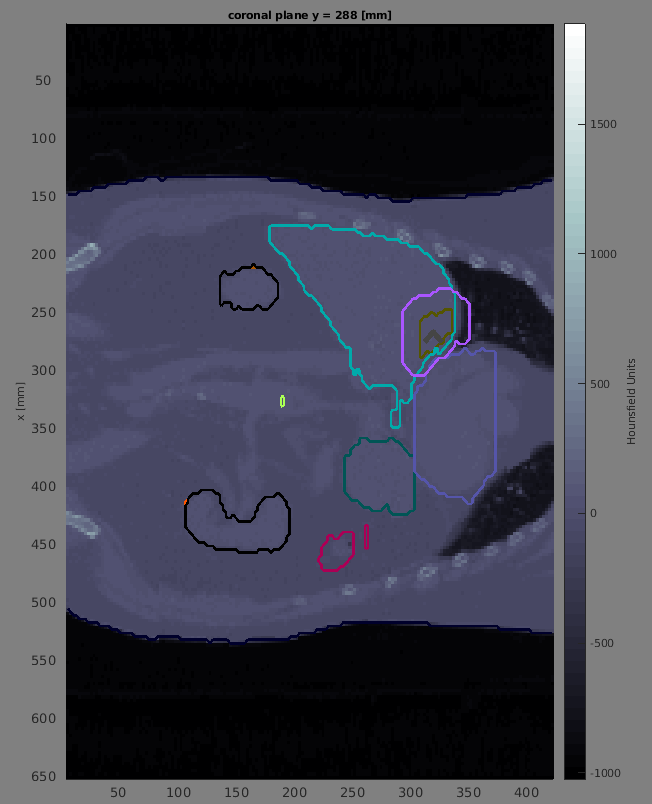
\includegraphics[height=.2\textheight]{./Figures/LiverCoronal} 
  
  On remarque notamment que le coeur est pratiquement dans le même plan axial que le volume cible planifié (PTV).
\end{reponse}


\question Pour se faire une idée du traitement appliqué par défaut avec ce fantôme, relever (sans rien modifier) le nombre de fractions prévues et les critères d'optimisation (\g{objectives \& constraints}, c'est-à-dire la dose prescrite pour irradier la tumeur, la dose maximale à déposer dans les organes à risque (OAR) (donner les valeurs par fraction) ainsi que les \g{fonctions de coût} (colonne \g{obj./const.}).

\begin{reponse}
  \begin{itemize}
		\item Nombre de fractions : 30
    \item Tumeur : 45~Gy (1,5~Gy par fraction) avec une fonction de coût \g{squared deviation}
    \item OAR : 25~Gy (0,8~Gy par fraction) avec une fonction de coût \g{squared overdose}
  \end{itemize}

\end{reponse}

\subsection{Champ d'irradiation unique}

On cherche à comparer les distributions de dose et les histogrammes \g{Dose-Volume} obtenus avec un champ d'irradiation de photons, protons et d'ions carbone. 

\question \label{1champ} Pour chaque type de rayonnement (photons, protons et ions carbone) :
\begin{itemize}
  \item choisir le \textbf{Radiation Mode} et définir l'angle du faisceau à 0° (gantry angle) en laissant les critères d'optimisation inchangés (\g{objectives \& constraints}) ;
  \item déclencher le calcul de la dose via le bouton \textbf{\g{Calc. Influence Mx}} et lancer l'optimisation inverse en cliquant sur \textbf{\g{Optimize}};
  \item observer les distributions de dose résultante avec la vue axiale. \textbf{Faire des captures d'écran et les mettre côte à côte pour les comparer.}
  \item cliquer enfin sur le bouton \textbf{\g{Show DVH}} pour afficher les histogrammes \g{Dose-Volume} (HDV) et cliquer sur l'icône \g{disquette} pour enregistrer ces histogrammes sous formes de fichiers \texttt{.fig} dans le dossier d'analyse (\texttt{masterclass/MasterclassPT\_Notebook}). Ces fichiers seront analysés dans un second temps.
\end{itemize}

\begin{reponse}

Les distributions de dose axiales obtenues avec des champ d'irradiation \g{Photons}, \g{Protons} et \g{Ions carbone} à 0°.

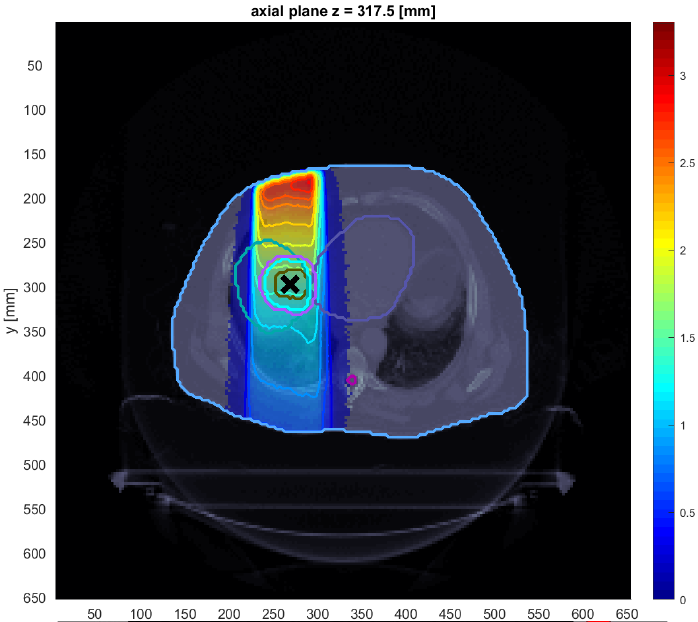
\includegraphics[width=.3\textwidth]{./Figures/Photons0_DistriDose_Axial} \quad 
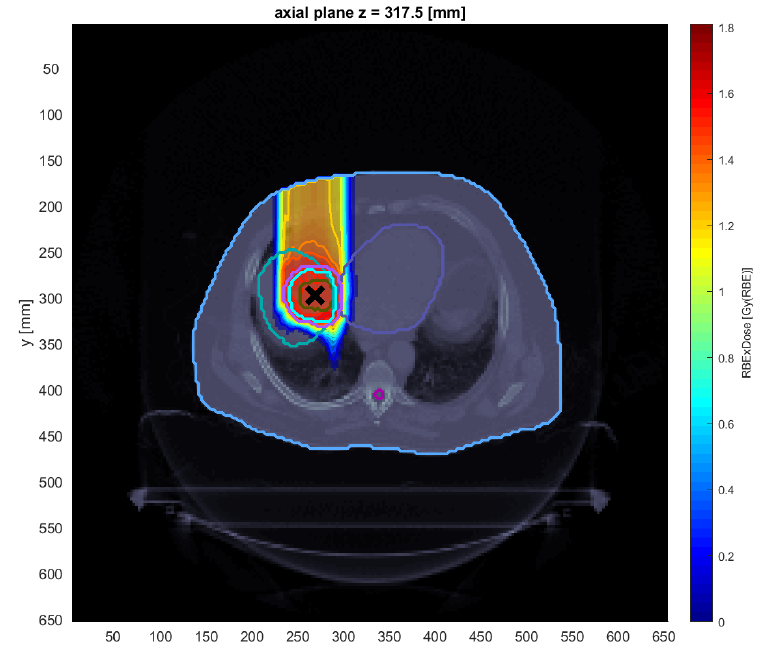
\includegraphics[width=.3\textwidth]{./Figures/Protons0_DistriDose_Axial} \quad 
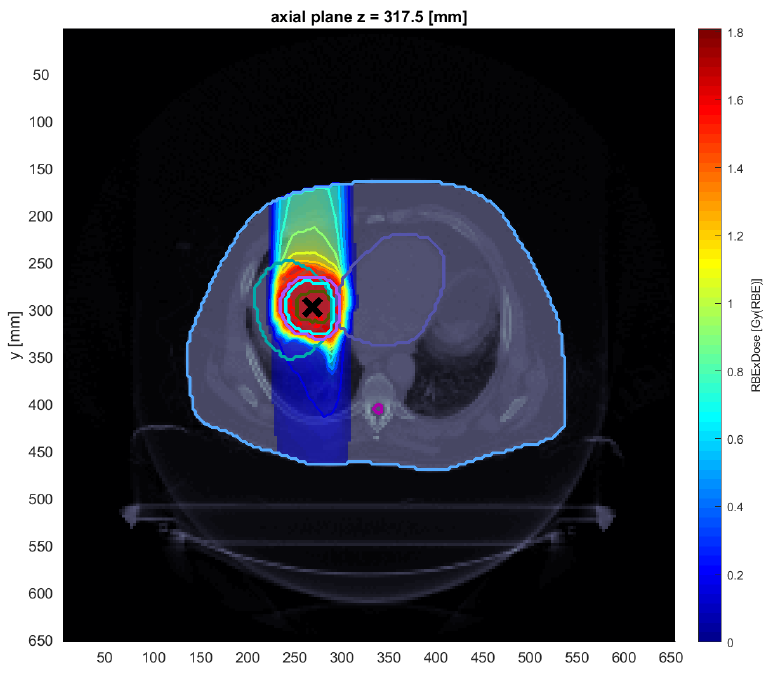
\includegraphics[width=.3\textwidth]{./Figures/Carbone0_DistriDose_Axial} \quad 

\end{reponse}

\question Analyser les fichiers (HDV) en exécutant le jupyter notebook :
\begin{itemize}
  \item se mettre dans le dossier \texttt{masterclass/MasterclassPT\_Notebook}
  \item taper dans un terminal: \texttt{jupyter-notebook masterclass.ipynb \&}
\end{itemize}

Nota Bene : penser à adapter le nom des fichiers de données dans le notebook en fonction des noms de fichier que vous avez choisis au moment de leur enregistrement. Mettre les figures HDV côté à côte et les comparer. Relever les grandeurs suivantes fournies par le notebook :
\begin{itemize}
  \item la fraction du volume tumoral avec moins de 95\% de la dose prescrite (\g{écart tumeur})
  \item la fraction du volume des 2 organes à risque (OAR) recevant plus que la dose maximale prévue dans l'optimisation de traitement (\g{écart OAR}).
\end{itemize}

\begin{reponse}

	Les DHV obtenus avec des photons, protons et des ions carbone (de gauche à droite) avec un champ d'irradiation à 0°.

	\includegraphics[width=.3\textwidth]{../Analysis/Photons} \quad 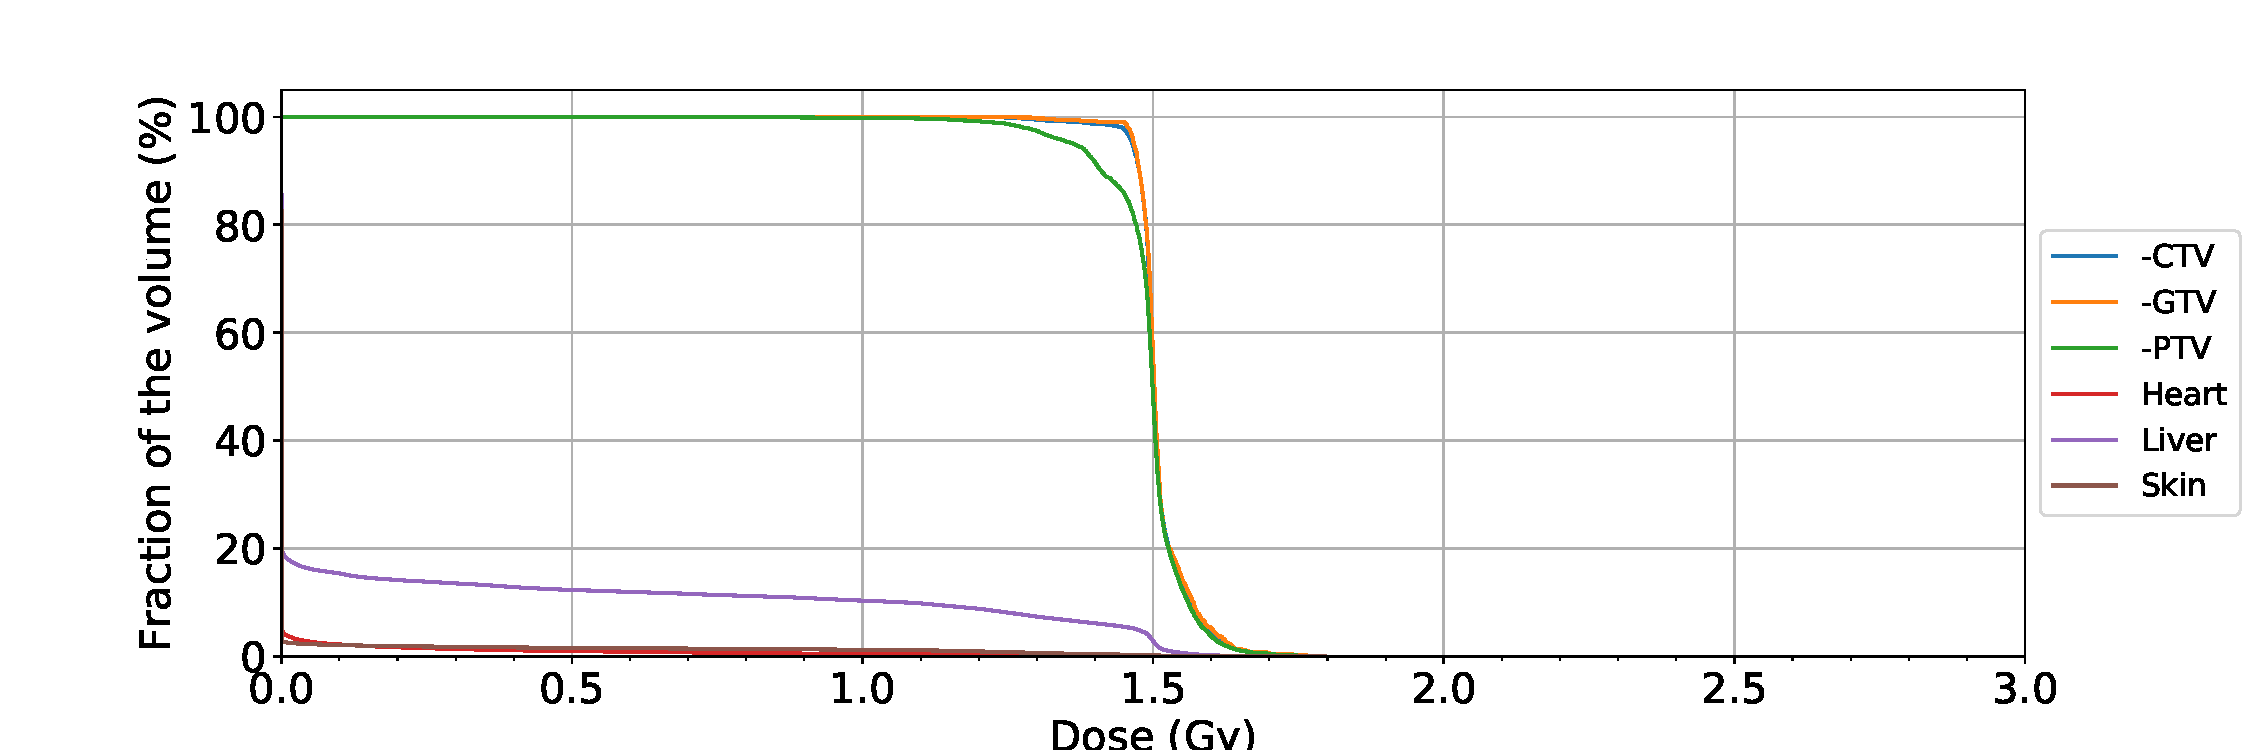
\includegraphics[width=.3\textwidth]{../Analysis/Protons0}  \quad 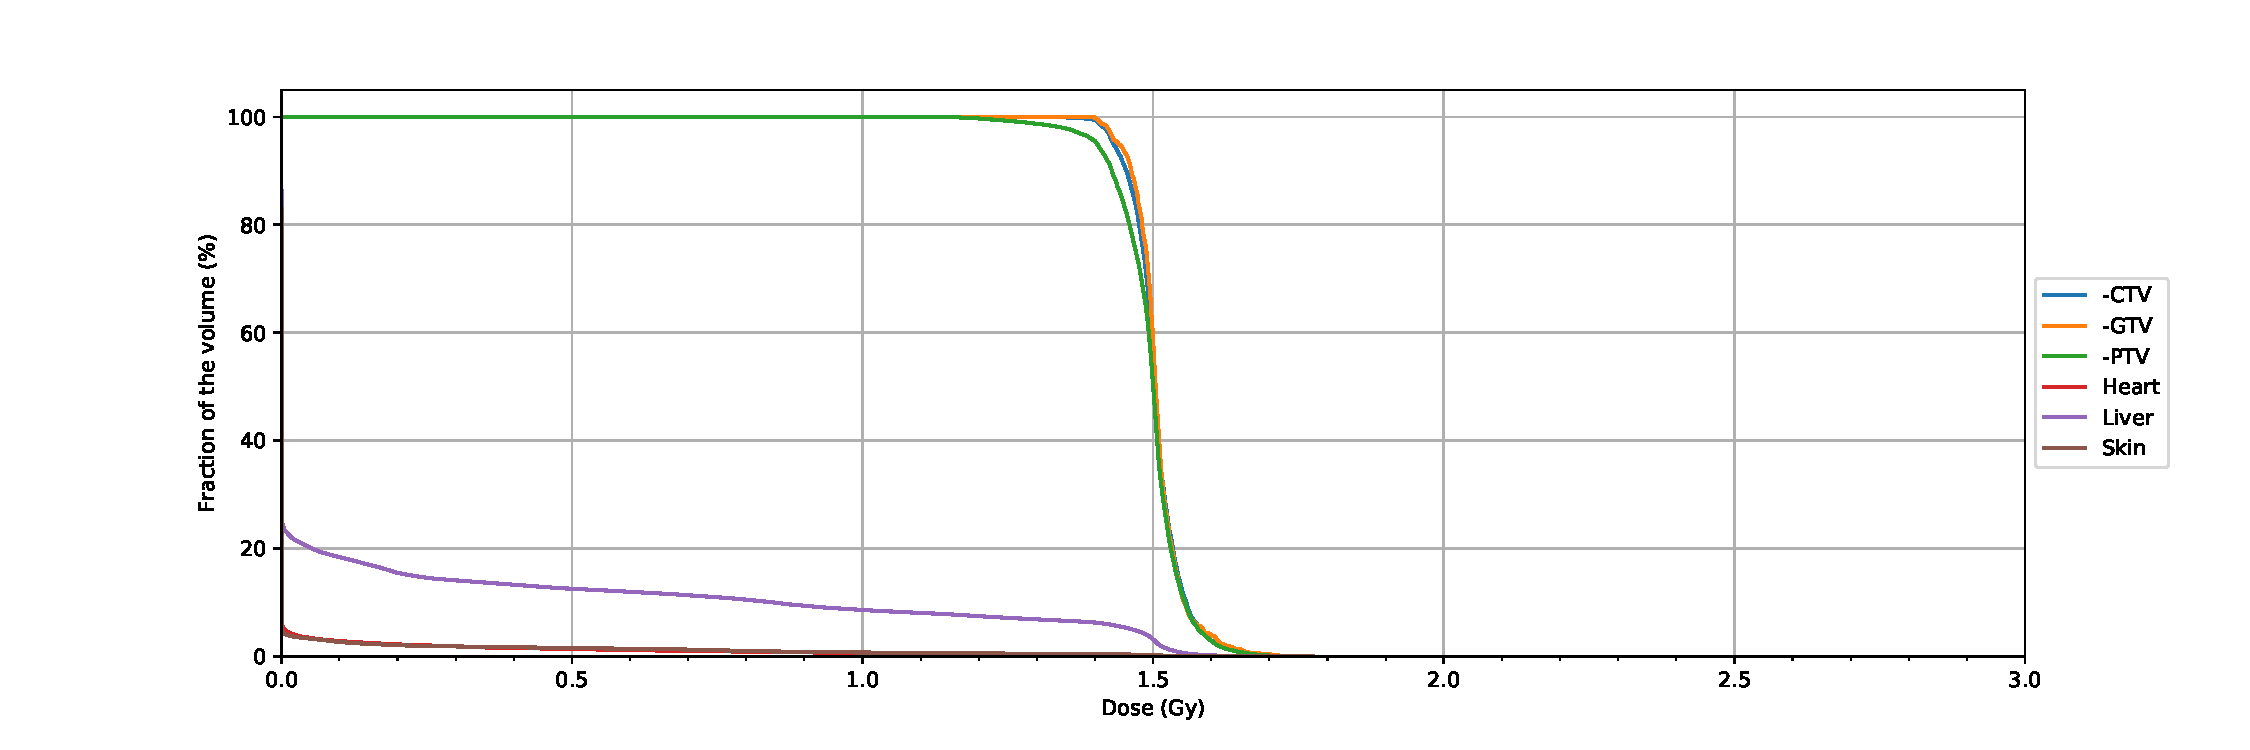
\includegraphics[width=.3\textwidth]{../Analysis/Carbon0}  

	\begin{tabular}{|l|c|c|c|}
    \hline
						& \g{écart tumeur}	& \g{écart foie} & \g{écart coeur}\\
		\hline
			Photons & 38,7\% & 14,9\%	& 1,1\%\\
    \hline    
			Protons & 11,4\% & 11,1\%	& 0,6\\
    \hline    
			Ions carbone & 9,0\% & 10,1\%& 0,8\%\\
    \hline        
  \end{tabular} 

\end{reponse}

\subsection{Champs d'irradiation multiples avec des photons}

On cherche maintenant à utiliser plusieurs champs d'irradiations \g{Photons} pour tendre vers une planification de traitement réaliste. 

\question Définir un plan de traitement avec 5 champs d'irradiations avec un espacement équidistant des angles de faisceau (Gantry Angle) : 0 72 144 216 288. On prendra un angle de table de traitement (Couch Angle) constant et égal à 0, c'est-à-dire : 0 0 0 0 0. 
\begin{itemize}
  \item observer les distributions de dose résultante avec la vue axiale. \textbf{Faire des captures d'écran et les mettre côte à côte pour les comparer.}
  \item cliquer enfin sur le bouton \textbf{\g{Show DVH}} pour afficher les histogrammes \g{Dose-Volume} (HDV). Enregistrer le fichier sous la forme d'un fichier \texttt{.fig}.
  \item Comparer les HDV obtenus avec 1 champ et 5 champs ainsi que les grandeurs suivantes : \g{écart tumeur}, \g{écart foie} et \g{écart c\oe ur} : 
  \begin{itemize}
    \item l'écart dans les organes à risque correspond à la fraction du volume de l'organe qui reçoit une dose supérieur à la dose max prévue dans la planification de traitement.
    \item l'écart dans la tumeur correspond à la fraction du volume tumoral qui reçoit une dose inférieure à 95\% de la dose prescrite.
  \end{itemize}
\end{itemize}

\begin{reponse}

	NB : l'angle de table de traitement égal à 0° présente l'avantage de minimiser la quantité de tissus sains à traverser pour atteindre la tumeur (champs d'irradiation dans un plan axial).
	
	La distribution de dose obtenue avec les 5 champs d'irradiation \g{photons} demandées est donnée sur la figure de droite suivante (la figure de gauche rappelle la distribution obtenue avec  un champ d'irradiation) :	
	
	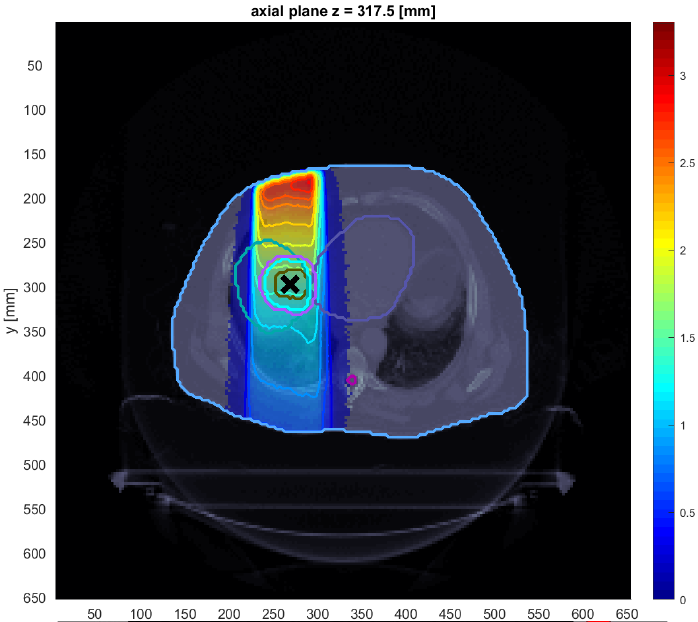
\includegraphics[width=.3\textwidth]{./Figures/Photons0_DistriDose_Axial} \quad
	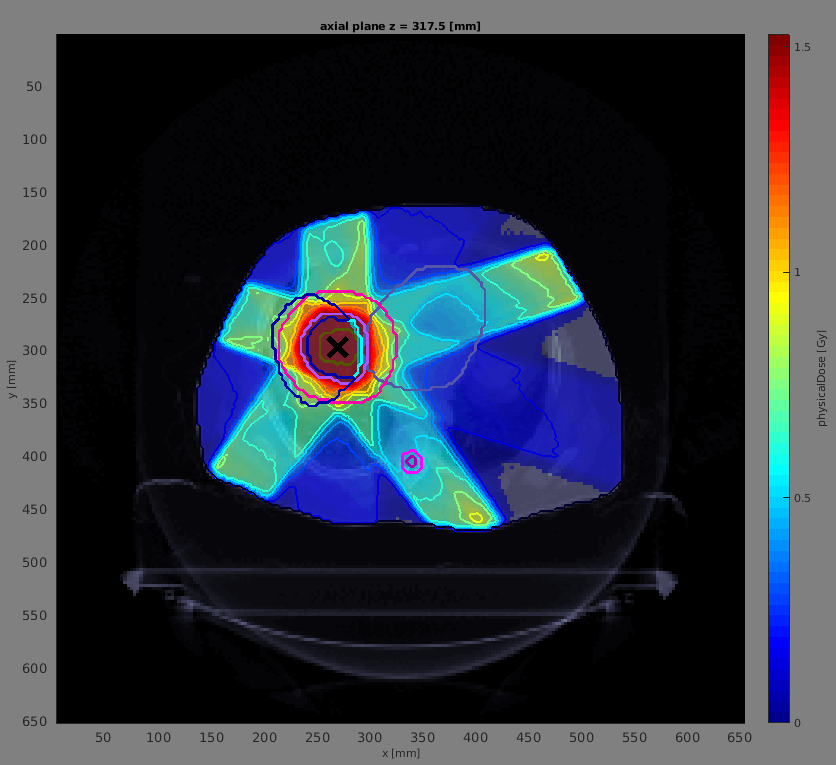
\includegraphics[width=.3\textwidth]{../Figures/Photons5ChampsEquiCouch0}
	
	On obtient les HDV suivants : 1 champ (à gauche) et 5 champs (à droite) :
	
	\includegraphics[width=.3\textwidth]{../Analysis/Photons} \quad 
	\includegraphics[width=.3\textwidth]{../Analysis/Photons5angEquiCouch0}
	
	\begin{tabular}{|l|c|c|c|}
    \hline
						& \g{écart tumeur}	& \g{écart foie} & \g{écart c\oe ur}\\
		\hline
			Photons 1 champ & 38,7\% & 14,9\%	& 1,1\%\\
    \hline    
			Photons 5 champs équidistants & 2,2\% & 11,8\%	& 3,9\%\\
    \hline        
  \end{tabular} 
  Le plan de traitement avec 5 champs est clairement nettement meilleur même s'il conduit à une dose légèrement plus importante dans le c\oe ur.
  
\end{reponse}

\question A faire plutôt en fin du TP en fonction du temps qu'il vous reste : essayer de changer les angles des champs d'irradiations pour améliorer la planification de traitement. Mettre vos résultats dans le fichier en ligne suivant : \url{https://lite.framacalc.org/masterclass-9zpo}. \\
Commencer avec 5 champs d'irradiations avant de réduire éventuellement le nombre de champs.



\end{questions}

\section{Impact des incertitudes de positionnements du patient sur des irradiations photons et protons (tumeur du cerveau)}
 
 L'objectif de cet exercice est d'observer l'impact d'un décalage du patient sur les distributions de dose photons et protons.
 
 \begin{itemize}
   \item[*] Charger un cas de patient atteint avec une tumeur à la tête (ALDERSON.mat) puis :
	\begin{itemize}
		\item choisir le \textbf{Radiation Mode} (Proton) et définir 3 angles de champs d'irradiation ;
		\item déclencher le calcul de la dose via le bouton \textbf{\g{Calc. Influence Mx}} et lancer l'optimisation inverse en cliquant sur \textbf{\g{Optimize}};
		\item observer les distributions de dose résultante avec la vue axiale. \textbf{Faire des captures d'écran et les mettre côte à côte pour les comparer.}
		\item cliquer enfin sur le bouton \textbf{\g{Show DVH}} pour afficher les histogrammes \g{Dose-Volume} (HDV) et cliquer sur l'icône \g{disquette} pour enregistrer ces histogrammes sous formes de fichiers \texttt{.fig}. 
	\end{itemize}
	\item[*] Simulez une erreur de positionnement du patient en décalant l'isocentre (l'origine du référentiel). Pour cela :
	\begin{itemize}
		\item décocher la case \g{auto} de l'iso-centre et définir un nouvel iso-centre décalé de 10 mm vers le tronc cérébral (\g{brainstem}), c'est-à-dire un isocentre à 155.4 127.3 186.4 ;
		\item recalculer la dose basée sur les intensités de faisceau de rayon optimisées précédemment en cliquant sur le bouton (\g{Recalc}). \textbf{Ne pas effectuer une nouvelle optimisation}. 
	\end{itemize}
 \end{itemize}

\begin{questions}

\question Comparer les distributions de dose (vue axiale) obtenues avec et sans erreur de positionnement ainsi que les HDV et différents \g{écarts} : \g{écart tumeur} et les 2 \g{écarts OAR} les plus élevés.

\begin{reponse}

	\begin{itemize}
	  \item Les distribution de dose sans puis avec erreur de positionnement \\
	  \includegraphics[width=.3\textwidth]{./Figures/ALDERSON_Protons0-60-240} \quad 
	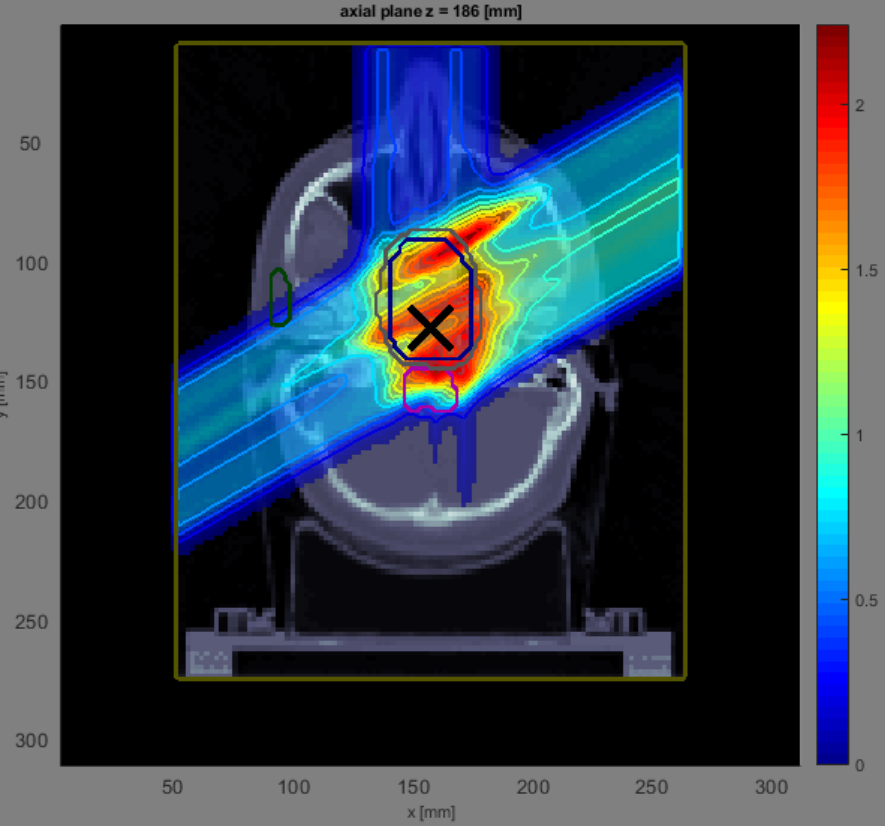
\includegraphics[width=.3\textwidth]{./Figures/ALDERSON_Protons0-60-240_shifted} 
		\item Les HDV sans puis avec erreur de positionnement \\
	  \includegraphics[width=.3\textwidth]{../Analysis/ALDERSON_Protons0-60-240} \quad 
	\includegraphics[width=.3\textwidth]{../Analysis/ALDERSON_Protons0-60-240_shift} 
		\item Les différents écarts : \g{écart tumeur}, écart tronc cérébral et écart lobe temporal gauche \\
		\begin{tabular}{|l|c|c|c|}
			\hline
										& \g{écart tumeur}	& \g{écart Brainstem} & \g{écart Temp(L)}\\
			\hline
				Sans décalage & 8,7\% & 11,4\%	& 3,8\%\\
			\hline    
				Avec décalage & 71,2\%\% & 37,0\%	& 5,1\%\\
			\hline        
		\end{tabular} 	
	\end{itemize}

\end{reponse}

\end{questions}

Le TP se termine par une séance de restitution pendant laquelle vous pourrez présenter vos résultats. Un template de présentation est disponible sur \href{https://docs.google.com/presentation/d/12wZ0YFja60zxPmlYEmSYEnNd9OQk_ws6j8wE14OOw50/edit#slide=id.p}{ce document en ligne}.





\end{document}
